\chapter{Datenbankschnittstelle: \gls{hibernate}}
Dieses Kapitel behandelt die Datenbankanbindung der Kochbuchanwendung.
\section{Object-Relational Mapping (ORM)}
\gls{hibernate} bietet die Möglichkeit relationale Datenbankstrukturen auf Java Objekte zu mappen. Betrachtet man das ER-Model der Datenbank (s. Abb. \ref{hib_erm}) und das UML Diagramm der Modellschicht (s. Abb. \ref{hib_uml}), fällt einem sofort die strukturelle Ähnlichkeit auf. \gls{hibernate} bietet die Möglichkeit mithilfe eines Mappings durch \acrshort{xml} Files die Modellschicht direkt auf das relationale Schema der Datenbank abzubilden.
\begin{figure}[htbp]
    \centering
    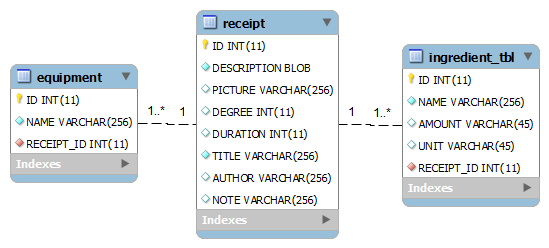
\includegraphics[scale=0.7]{images/relational-model.png}
    \caption{ER-Model der Kochbuch Datenbank}
    \label{hib_erm}
\end{figure}
\begin{figure}[htbp]
    \centering
    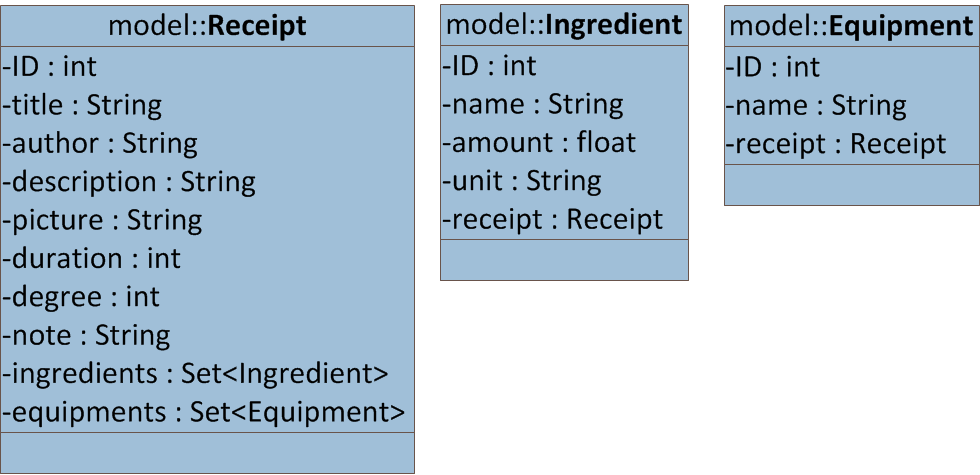
\includegraphics[scale=3.5]{images/model-uml.png}
    \caption{UML der Klassen der Modellschicht}
    \label{hib_uml}
\end{figure}

\section{Klassen - Tabellen Mapping}
Wie in Abbildung \ref{hib_erm} und \ref{hib_uml} zu sehen ist werden drei Klassen auf drei Tabellen abgebildet. Jeweils eine Klasse wird auf eine Tabelle abgebildet. ($Namentlich: Receipt \rightarrow receipt, Ingredient \rightarrow ingredient\_tbl \ und \  Equipment \rightarrow equipment$)
Das Mapping findet statt, indem für jede Klasse, die auf eine Tabelle abgebildet werden soll, eine \acrshort{xml} Konfigurationsdatei im selben package wie die Klasse angelegt wird, die dieses Mapping definiert. Heißt die Klasse \textit{"Foo.java"} ist der Name der Konfigurationsdatei \textit{"Foo.hbm.xml"}.
Sie sagt der Klasse auf welche Tabelle sie abgebildet wird. In diesem Mapping können dann Attribute und Relationen für diese Tabelle/Klasse definiert werden.

\section{Mapping einfacher Attribute}
Ein einfaches Attribut wird über das proberty Tag auf eine Tabellenspalte gemappt. Ein solches Beispielmapping eines Attributs sieht man in Quellcode \ref{hib_prop}. Das Attribut \textit{"name"} benennt das Attribut der Klasse. \textit{"column"} nennt die Spalte der Tabelle, auf die das Attribut, das durch \textit{"name"} definiert wird, gemappt wird. \textit{"type"} ist der Datentyp in dem das Attribut aus der Klasse gelesen und in der Datenbank gespeichert wird. Der Datentyp ist weder der der Javaklasse noch der Datentyp der Datenbanktabellenspalte. Es ist ein \gls{hibernate} mapping Typ.
Im Beispiel Quellcode \ref{hib_prop} ist außerdem, ein optionales Attribut \textit{"not-null"} zu sehen. Die vorherigen Attribute waren alle Pflichteingaben, auf die weitere optionale Attribute folgen können. \textit{not-null="true"} erlaubt es nur Werte ungleich null zu der Spalte hinzuzufügen.
\begin{lstlisting}[caption={Mapping eines Attributes},label=hib_prop]
    <property name="title" column="TITLE" type="string" not-null="true" />
\end{lstlisting}

\section{Mapping von Relationen}
In \gls{hibernate} gibt es zwei Möglichkeiten des Mappings für 1:n Beziehungen. Man kann das Mapping aus zwei Perspektiven sehen: one-to-many oder eine many-to-one Relation. In unserem Kochbuch sind die Rezepte 1:n mit den Zutaten verbunden. Es ist eine one-to-many Beziehung. Genauso könnte man sagen sind die Zutaten many-to-one mit den Rezepten verbunden.
So kann man die Beziehung wie in Beispiel Quellcode \ref{hib_otm} als one-to-many Beziehung von Rezepten zu Zutaten beschreiben. Die one-to-many Beziehung wird in der Klasse mithilfe eines HashSets dargestellt. In Hibernate werden Sets mit dem \textit{set} Tag dargestellt. Dieses HashSet wird hier mit dem \textit{"name"} Attribut angesprochen. \textit{"cascade"} und \textit{"lazy"} sind optionale Attribute und beschreiben das Verhalten bei Updates/Löschen (hier: Zutaten werden auch aktualisiert, wenn Rezepte aktualisiert wurden) oder versetzen Transaktionen mit einer Priorität (hier: nur Indizes des Sets werden geladen. Das Objekt selber wird erst bei Bedarf aus der Datenbank geladen. Für große Anwendungen bietet diese Option Performance-Vorteile).
Der Tag \textit{key} mit seinem Attribut \textit{"column"} beschreibt die Spalte in der Tabelle, in der die Relation als Fremdschlüssel gespeichert wird. Das \textit{one-to-many} Tag gibt mit seinem \textit{"class"} Attribut die Klasse in der sie referenziert wird an. Dadurch ist auch die Hibernate Konfigurationsdatei und darin die Tabelle in der Datenbank zu dieser Klasse bekannt.
\begin{lstlisting}[caption={One-To-Many Beziehung von Rezepten zu Zutaten},label=hib_otm]
    <set name="ingredients" cascade="all" lazy="true">
		<key column="RECEIPT_ID" />
		<one-to-many class="model.Ingredient" />
	</set>
\end{lstlisting}
Die andere Richtung beschreibt das Beispiel Quellcode \ref{hib_mto}. Das \textit{"name"} Attribut des \textit{many-to-one} Tags gibt den Namen des Attributs in der Klasse an, die den Fremdschlüssel als Objektreferenz speichert. Das \textit{"class"} Attribut gibt die Klasse auf die die Referenz zeigt an und entspricht dem Datentyp des Java Attributs. \textit{"column"} gibt die Spalte in der Datenbanktabelle an, in der die Referenz über einen Fremdschlüssel abgebildet wird. Nun kommt abschließend noch ein optionales Attribut \textit{"cascade"} und verhält sich wie in Beispiel Quellcode \ref{hib_otm} beschrieben: Bei Updates oder Löschen des referenzierten Tabelle (Rezept) kaskadiert die Aktion. Die Zutaten werden ebenfalls aktualisiert/gelöscht.
\begin{lstlisting}[caption={Many-To-One Beziehung von Zutaten zu Rezepten},label=hib_mto]
    <many-to-one name="receipt" class="model.Receipt" column="RECEIPT_ID" cascade="all" />
\end{lstlisting}

\subsection*{Die Unterschiede der Relationen}
1:1 Relationen verbinden eine Zeile einer Tabelle mit einer Zeile einer anderen Tabelle.
Sobald eine Zeile einer Tabelle mit mehreren Zeilen einer anderen Tabelle verbindet ist es eine 1:n Relation. Bei n:m Relationen werden mehrere Zeilen der einen Tabelle mit mehreren Zeilen einer anderen Tabelle verbunden. Da diese Information jedoch nicht mehr in einer Spalte sinnvoll gespeichert werden kann, benötigt man eine extra Tabelle um diese Verbindungsinformationen zu speichern.

In Hibernate ist dies ebenfalls so. Durch die one-to-one, one-to-many, many-to-one und many-to-many Tags können diese Relationen auch über Hibernate abgebildet werden.

\section{Bidirektionales Mapping}
Indem eine Relation in beiden Konfigurationsdateien definiert wird, macht man die beiden Tabellen bidirektional bekannt. Das bedeutet, dass ein Update eines Objektes, dass auf eine dieser Tabellen abgebildet ist, auch die anderen Objekte, die zu dieser Relation gehören, ebenfalls aktualisiert. So genügt es auch beim Einfügen in die Tabelle eines der Objekte der Relation hinzuzufügen. Würde man die Tabellen nicht bidirektional bekannt machen, wäre dies eine mögliche Fehlerquelle im späteren Programmieren der Anwendung. Durch bidirektionales Verknüpfen wird diese Fehlerquelle konzeptionell vermieden.

